\documentclass[manuscript,screen,review]{acmart}

%% ACM metadata
\copyrightyear{2025}
\acmYear{2025}
\acmConference[RecSys '25]{Nineteenth ACM Conference on Recommender Systems}{October 6--10, 2025}{Chongqing, China}

%% Additional packages (not bundled in acmart)
\usepackage{tikz-cd}
\usepackage{multicol}

%%% Title
\title{POI-Centric Hierarchical Note-Based User Memory with Dynamic Routing and Trait Elevation}

%%% Authors (single-blind for Industry Track)
\author{Junguel Lee}
\affiliation{%
  \institution{Naver Corp}
  \country{South Korea}
}
\email{junguel.lee@navercorp.com}

\author{Jungseok Lee}
\affiliation{%
  \institution{Naver Corp}
  \country{South Korea}
}
\email{jungseok.lee@navercorp.com}

\begin{abstract}
Modeling user place preferences from large-scale POI (Point-of-Interest) interaction logs requires capturing fine-grained behavioral signals while organizing them into structured, updateable representations that evolve over time.
Recent memory-augmented LLM agents~\cite{mem0,amem,personamem-v2} have shown that structured memory can outperform both full-context approaches~\cite{beyond-context-window} and flat retrieval systems for personalization tasks.
We propose a \textbf{POI-centric Hierarchical Note-based Memory}, a structured memory architecture that transforms raw place interaction logs into dynamically maintained, multi-level preference representations.
Building on the hierarchical memory paradigm established by PersonaMem-v2~\cite{personamem-v2}, our approach introduces three key extensions:
(1)~\textbf{dynamic hierarchical routing}, where an LLM maps extracted preferences to existing or newly created taxonomy paths while enforcing level-consistency constraints;
(2)~\textbf{common trait elevation}, a novel backward-pass operation that promotes shared attributes from sibling notes to their parent, reducing redundancy through hierarchical compression; and
(3)~\textbf{three-axis preference separation}, which isolates demographics, explicit preferences, and implicit behavioral signals into distinct channels with root-exclusive demographic routing.
Unlike flat log retrieval or chunk-based memory systems, our approach consolidates distributed implicit~\cite{proex} and explicit~\cite{deeper} POI signals into topic-specific notes organized within a hierarchy grounded in a POI taxonomy.
This enables preference modeling at multiple abstraction levels, ranging from fine-grained subcategory interests (e.g., specific food types) to higher-level behavioral tendencies (e.g., dining-focused lifestyle patterns).
To ensure temporal consistency and structural integrity, we introduce a Memory Agent that autonomously manages the lifecycle of notes through two complementary processes: (1)~forward aggregation of new POI interaction signals into appropriate nodes and (2)~backward consolidation, conflict resolution, and pruning to prevent redundancy and preference drift.
We further propose a POI-domain evaluation framework inspired by PersonaGym~\cite{personagym} that quantitatively measures alignment between hierarchical memory representations and real user behavioral patterns.
Experimental results demonstrate that the proposed POI-centric hierarchical memory produces more coherent, adaptive, and human-aligned user place personas compared to full-context, flat-memory, and fixed-hierarchy baselines.
\end{abstract}

\begin{document}
\maketitle


%% ============================================================
%% INTRODUCTION
%% ============================================================
\section{Introduction}

Personalization is a core competitive advantage of modern platform services, directly improving user satisfaction and click-through rate (CTR). In POI (Point-of-Interest)-centric services such as place recommendation, accurately understanding users' preferred place types and visitation patterns is crucial to service quality. This requires precise modeling of each user's unique preferences and behavioral tendencies. Prior work typically constructs user personas by either injecting the full interaction history into the context of a large language model (LLM)~\cite{beyond-context-window} or by chunking the history and retrieving relevant pieces via similarity~\cite{dpr,contriever}. The resulting personas serve as user context in recommendation and search, and their quality is a key driver of personalization performance.

However, generating high-quality place-preference personas from real-world POI activity logs is fundamentally challenging. User logs (search, save, click, visit, reservation) are large-scale and continually expanding, and they include substantial exploratory or noisy behavior that does not explicitly reveal preferences. Moreover, place preferences often emerge gradually from accumulated interactions rather than being observable from any single log entry. Explicit signals such as reviews or blog posts directly express preferences~\cite{deeper}, but they are sparse and limited to a subset of users. In contrast, implicit behaviors---repeated clicks on POIs within a category, sustained exploration of similar places, or prolonged dwell time on venue pages---are pervasive~\cite{proex}. While any single implicit signal may be ambiguous, consistent patterns across multiple interactions can reveal structured latent preferences.

Because place preferences evolve over time, a mechanism is also required to reconcile conflicts between historical patterns and current interests. These characteristics expose limitations of existing persona construction methods. Feeding the full interaction history into an LLM quickly reaches context-length limits and can suffer from lost-in-the-middle effects~\cite{lost-in-the-middle} that dilute salient preference signals. Even with recent advances in long-context models, empirical evidence shows that full-context approaches achieve strong factual recall (92.85\% on LoCoMo~\cite{beyond-context-window}) but underperform structured memory systems for implicit personalization tasks (45.6\% vs.\ 55.2\%~\cite{personamem-v2}), while incurring substantially higher computational costs. Chunking the history and retrieving relevant segments via RAG mitigates length constraints, but in POI settings where preference signals are distributed across many logs, chunking further fragments already sparse evidence. Additionally, flat chunk structures make it difficult to flexibly move between fine-grained category preferences (e.g., Korean, Japanese, or caf\'{e}s) and higher-level tendencies such as a dining-focused lifestyle.

Recent work on memory-augmented LLM agents has begun to address these challenges. Mem0~\cite{mem0} maintains a flat list of memory items with ADD/UPDATE/DELETE operations and hash-based deduplication, but lacks hierarchical organization. A-Mem~\cite{amem} introduces structured notes with cross-node activation (``Aha Moments''), enabling inter-category linking but without explicit hierarchy management. PersonaMem-v2~\cite{personamem-v2} proposes a three-level hierarchical tree with dual extraction of explicit and implicit signals, demonstrating that structured memory outperforms full-context baselines for personalization. However, PersonaMem-v2 relies on fixed, predefined category slots and does not perform structural maintenance operations such as trait promotion across hierarchy levels. In the POI recommendation domain specifically, ZeroPOIRec~\cite{zeropoirec} demonstrates that LLM-generated personas can enable zero-shot POI recommendation through multi-aspect profiling (temporal, geographic, individual), validating the persona-based approach for place services.

\begin{figure}[t]
  \centering
  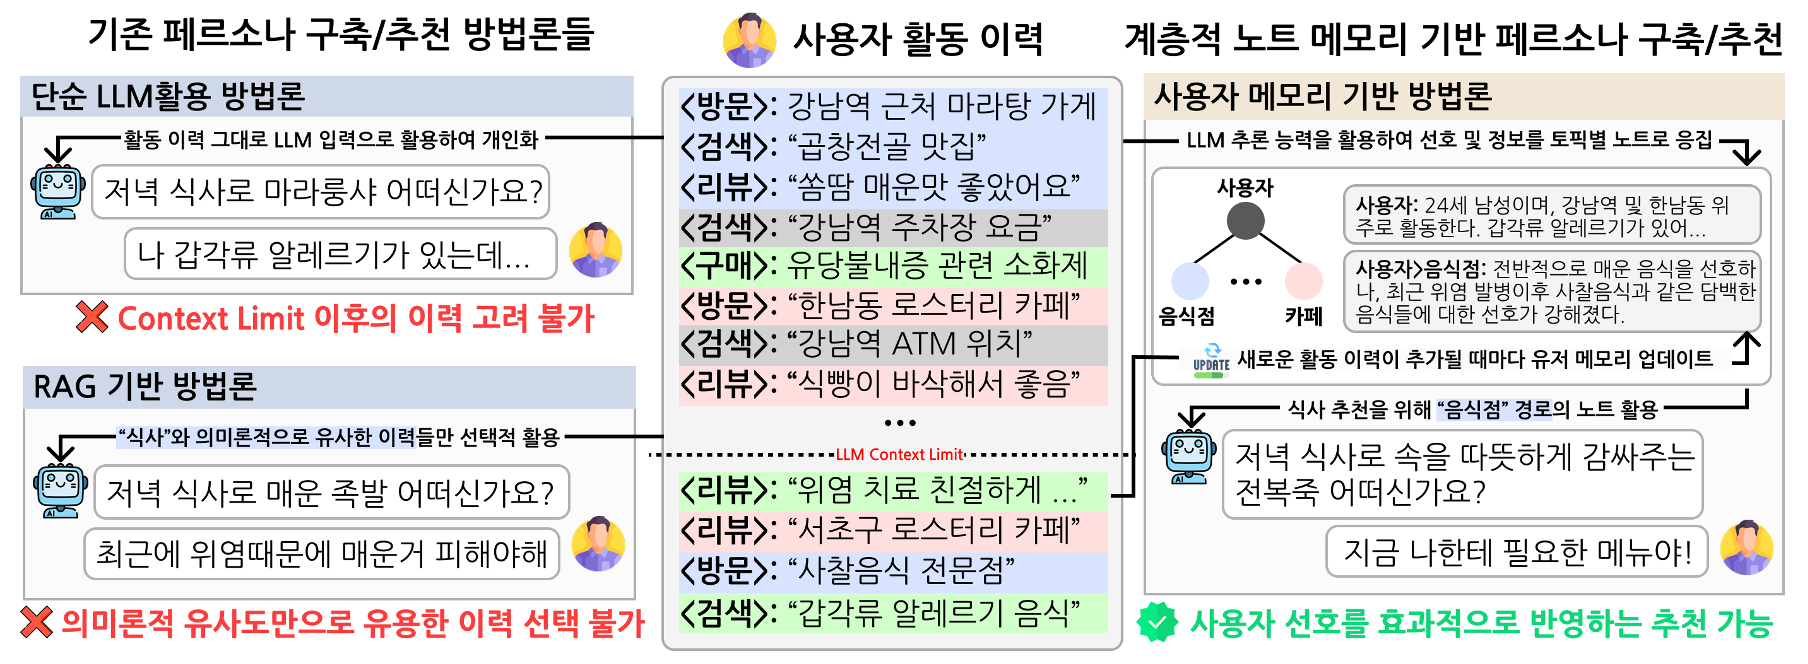
\includegraphics[width=\linewidth]{figures/method-comparison.png}
  \caption{Comparison of persona construction approaches. Existing methods either inject the full interaction history into an LLM context (top-left) or retrieve chunked logs via RAG (bottom-left), both of which struggle with scale, noise, and cross-session preference aggregation. Our proposed hierarchical note memory (right) consolidates user activity into structured, taxonomy-grounded notes and constructs context-adaptive personas through selective path reading.}
  \label{fig:comparison}
\end{figure}

\begin{figure}[t]
  \centering
  \includegraphics[width=\linewidth]{figures/overview.png}
  \caption{Overview of the POI-centric hierarchical note memory and its maintenance workflow. The Memory Agent performs forward aggregation (signal extraction $\rightarrow$ hierarchical routing $\rightarrow$ note update) and backward consolidation (sibling merging $\rightarrow$ common trait elevation $\rightarrow$ stale pruning).}
  \label{fig:overview}
\end{figure}

We address these challenges by proposing a POI-centric Hierarchical Note-based Memory and a Memory Agent that dynamically maintains it. The proposed memory aggregates preference signals from POI activities (search, save, click, visit, reservation) into topic-specific notes using LLM reasoning, consolidating implicit preferences dispersed across multiple logs into refined units. These notes are then organized within a hierarchy grounded in a POI taxonomy, enabling structured management of preferences from high-level domains down to subcategory granularity. This design supports context-adaptive persona construction by selectively utilizing preference information at the appropriate abstraction level for a given recommendation scenario (e.g., region-based, category-based, or situation-based).

This motivation is threefold: (i)~\textbf{category-wise trait separation}, which disentangles domain- and subcategory-specific preferences; (ii)~\textbf{update localization}, which confines incremental edits to only the notes affected by newly arrived interactions; and (iii)~\textbf{efficient information retrieval and management}, enabled by path-level access and hierarchy-aware maintenance operations.

Our contributions are as follows:
\begin{itemize}
    \item We propose a POI-centric hierarchical note memory that extends the hierarchical memory paradigm~\cite{personamem-v2} with \textbf{dynamic hierarchical routing}---an LLM-driven path mapping mechanism that reuses existing taxonomy paths or creates new ones while enforcing level-consistency constraints, unlike the fixed-slot approach of prior work.
    \item We introduce \textbf{common trait elevation}, a novel backward-pass operation that identifies shared attributes across sibling notes and promotes them to the parent node, achieving hierarchical compression analogous to minimizing description length across the tree. To our knowledge, this operation has not been proposed in prior memory systems~\cite{mem0,amem,personamem-v2}.
    \item We design a \textbf{three-axis preference separation} scheme that isolates user demographics (root-exclusive), explicit stated preferences, and implicit behavioral signals into distinct channels, providing cleaner information routing than the two-axis approach of PersonaMem-v2~\cite{personamem-v2}.
    \item We propose a POI-domain evaluation framework adapted from PersonaGym~\cite{personagym} and validate through experiments that the proposed memory outperforms full-context, flat-memory, and fixed-hierarchy baselines on persona quality and downstream recommendation metrics.
\end{itemize}


%% ============================================================
%% RELATED WORK
%% ============================================================
\section{Related Work}

\subsection{Memory-Augmented LLM Agents}

As large language models are increasingly deployed as autonomous agents, the need for persistent memory beyond the context window has driven a line of work on memory architectures. These systems vary along two axes: memory \textit{structure} (flat vs.\ hierarchical) and \textit{maintenance strategy} (append-only vs.\ actively managed).

\textbf{Flat memory systems.}
Mem0~\cite{mem0} maintains an unstructured list of memory items and applies per-item ADD, UPDATE, DELETE, and NO\_CHANGE operations when new information arrives, using hash-based deduplication to detect redundant entries. While effective for factual recall, the flat structure makes it difficult to represent preferences at multiple abstraction levels or to perform structural operations like trait generalization. MemGPT~\cite{memgpt} extends the context window through a virtual paging mechanism but does not impose semantic organization on stored content.

\textbf{Structured and hierarchical memory.}
A-Mem~\cite{amem} organizes notes in a Zettelkasten-inspired structure and introduces ``Aha Moments''---cross-node activation links that capture relationships between thematically distant notes. Their ablation shows that removing linking drops multi-hop F1 from 27.02 to 9.65, demonstrating the value of inter-node connections. However, A-Mem does not enforce a taxonomy-grounded hierarchy and lacks explicit maintenance operations for structural integrity (e.g., trait promotion or sibling consolidation).
EMem~\cite{emem} introduces expectation-guided selective storage, becoming the first memory system to outperform full-context approaches on the LoCoMo benchmark (78.0\% vs.\ 72.3\%), while using approximately 32$\times$ fewer tokens. This result validates that structured memory can match or exceed full-context quality when the storage mechanism is sufficiently selective.

PersonaMem~\cite{personamem} and its successor PersonaMem-v2~\cite{personamem-v2} are the most closely related systems to ours. PersonaMem-v2 proposes a three-level hierarchical tree (User $>$ Aspect $>$ Sub-aspect) with dual extraction of explicit and implicit signals, and demonstrates that this structure outperforms full-context baselines for personalization tasks (55.2\% vs.\ 45.6\% win rate with 16$\times$ fewer tokens). Our work extends this paradigm in three directions: we replace fixed category slots with dynamic LLM-driven routing, introduce common trait elevation as a backward-pass maintenance operation, and add a third extraction axis for demographic information with root-exclusive routing.

\subsection{LLM-Based Persona Generation and Evaluation}

The use of LLMs for constructing and evaluating user personas has been explored from both generation and benchmarking perspectives.
PersonaHub~\cite{personahub} demonstrates scalable persona synthesis from web text, producing over 1 billion diverse persona descriptions through text-to-persona and persona-to-persona generation methods.
DEEPER~\cite{deeper} focuses on dense persona extraction from user reviews for recommendation, producing structured preference representations from explicit user-authored content---a pipeline analogous to our explicit signal extraction stage.
SynthesizeMe~\cite{synthesizeme} proposes profile-conditioned synthetic data generation for personalization, while ProEx~\cite{proex} extracts expert-level preferences from implicit behavioral signals through multi-stage chain-of-thought reasoning.

On the evaluation side, PersonaGym~\cite{personagym} provides a dynamic evaluation framework with 200 personas across 10,000 questions spanning six dimensions (toxicity, persona adherence, conversational quality, linguistic habits, persona consistency, action justification). PersonaBench~\cite{personabench} evaluates multi-turn persona consistency. Our evaluation framework adapts the PersonaGym methodology to the POI domain, generating persona-conditioned preference prediction tasks grounded in actual user behavioral data.

\subsection{LLM-Based POI Recommendation}

LLM-based approaches to POI recommendation have demonstrated the potential of persona-driven place understanding.
ZeroPOIRec~\cite{zeropoirec} enables zero-shot POI recommendation by constructing LLM-generated user personas along three aspects---temporal patterns, geographic mobility, and individual characteristics---and using them to predict place preferences without interaction history at inference time. This validates the persona-based approach for POI services but operates statelessly, regenerating personas from scratch rather than maintaining persistent memory.
ProEx~\cite{proex} introduces multi-profile preference extraction with an invariant learning mechanism for recommendation, but focuses on single-session extraction rather than cumulative memory.
Persona-DB~\cite{persona-db} proposes retrieval-based persona selection from a database for response prediction, demonstrating the value of structured persona storage.
RMM~\cite{rmm} combines dense and sparse retrieval for memory-augmented dialogue, providing a hybrid retrieval strategy reference.

Our approach differs from these systems by maintaining a \textit{persistent, evolving} memory that accumulates evidence across sessions and supports structural maintenance, rather than performing one-shot extraction or stateless retrieval.

\subsection{Full-Context vs.\ Structured Memory}

The trade-off between full-context processing and structured memory is a central design decision for LLM-based personalization.
``Beyond the Context Window''~\cite{beyond-context-window} provides the most direct comparison: long-context GPT-5-mini achieves 92.85\% accuracy on the LoCoMo factual QA benchmark, substantially outperforming memory systems (Mem0: 57.68\%, MemGPT: 48.23\%). However, this advantage is specific to factual recall tasks where the answer appears verbatim in the history.

For implicit personalization---where preferences must be \textit{inferred} from behavioral patterns rather than directly retrieved---the picture reverses. PersonaMem-v2~\cite{personamem-v2} demonstrates that agentic memory achieves a 55.2\% win rate with approximately 2K tokens against full-context processing at 32K tokens (45.6\%). This gap is especially pronounced for POI preference modeling, where signals are distributed across hundreds of click/save events and individual actions are ambiguous. In our setting, implicit extraction averages 73K tokens per user---well beyond practical context limits for per-user processing and prohibitively expensive at scale.

These findings motivate our architectural choice: structured hierarchical memory for production POI personalization, with full-context serving as a quality validation baseline rather than a deployment strategy.


%% ============================================================
%% PROPOSED METHOD
%% ============================================================
\section{Proposed Method}

\subsection{Overview}

\begin{figure*}[t]
  \centering
  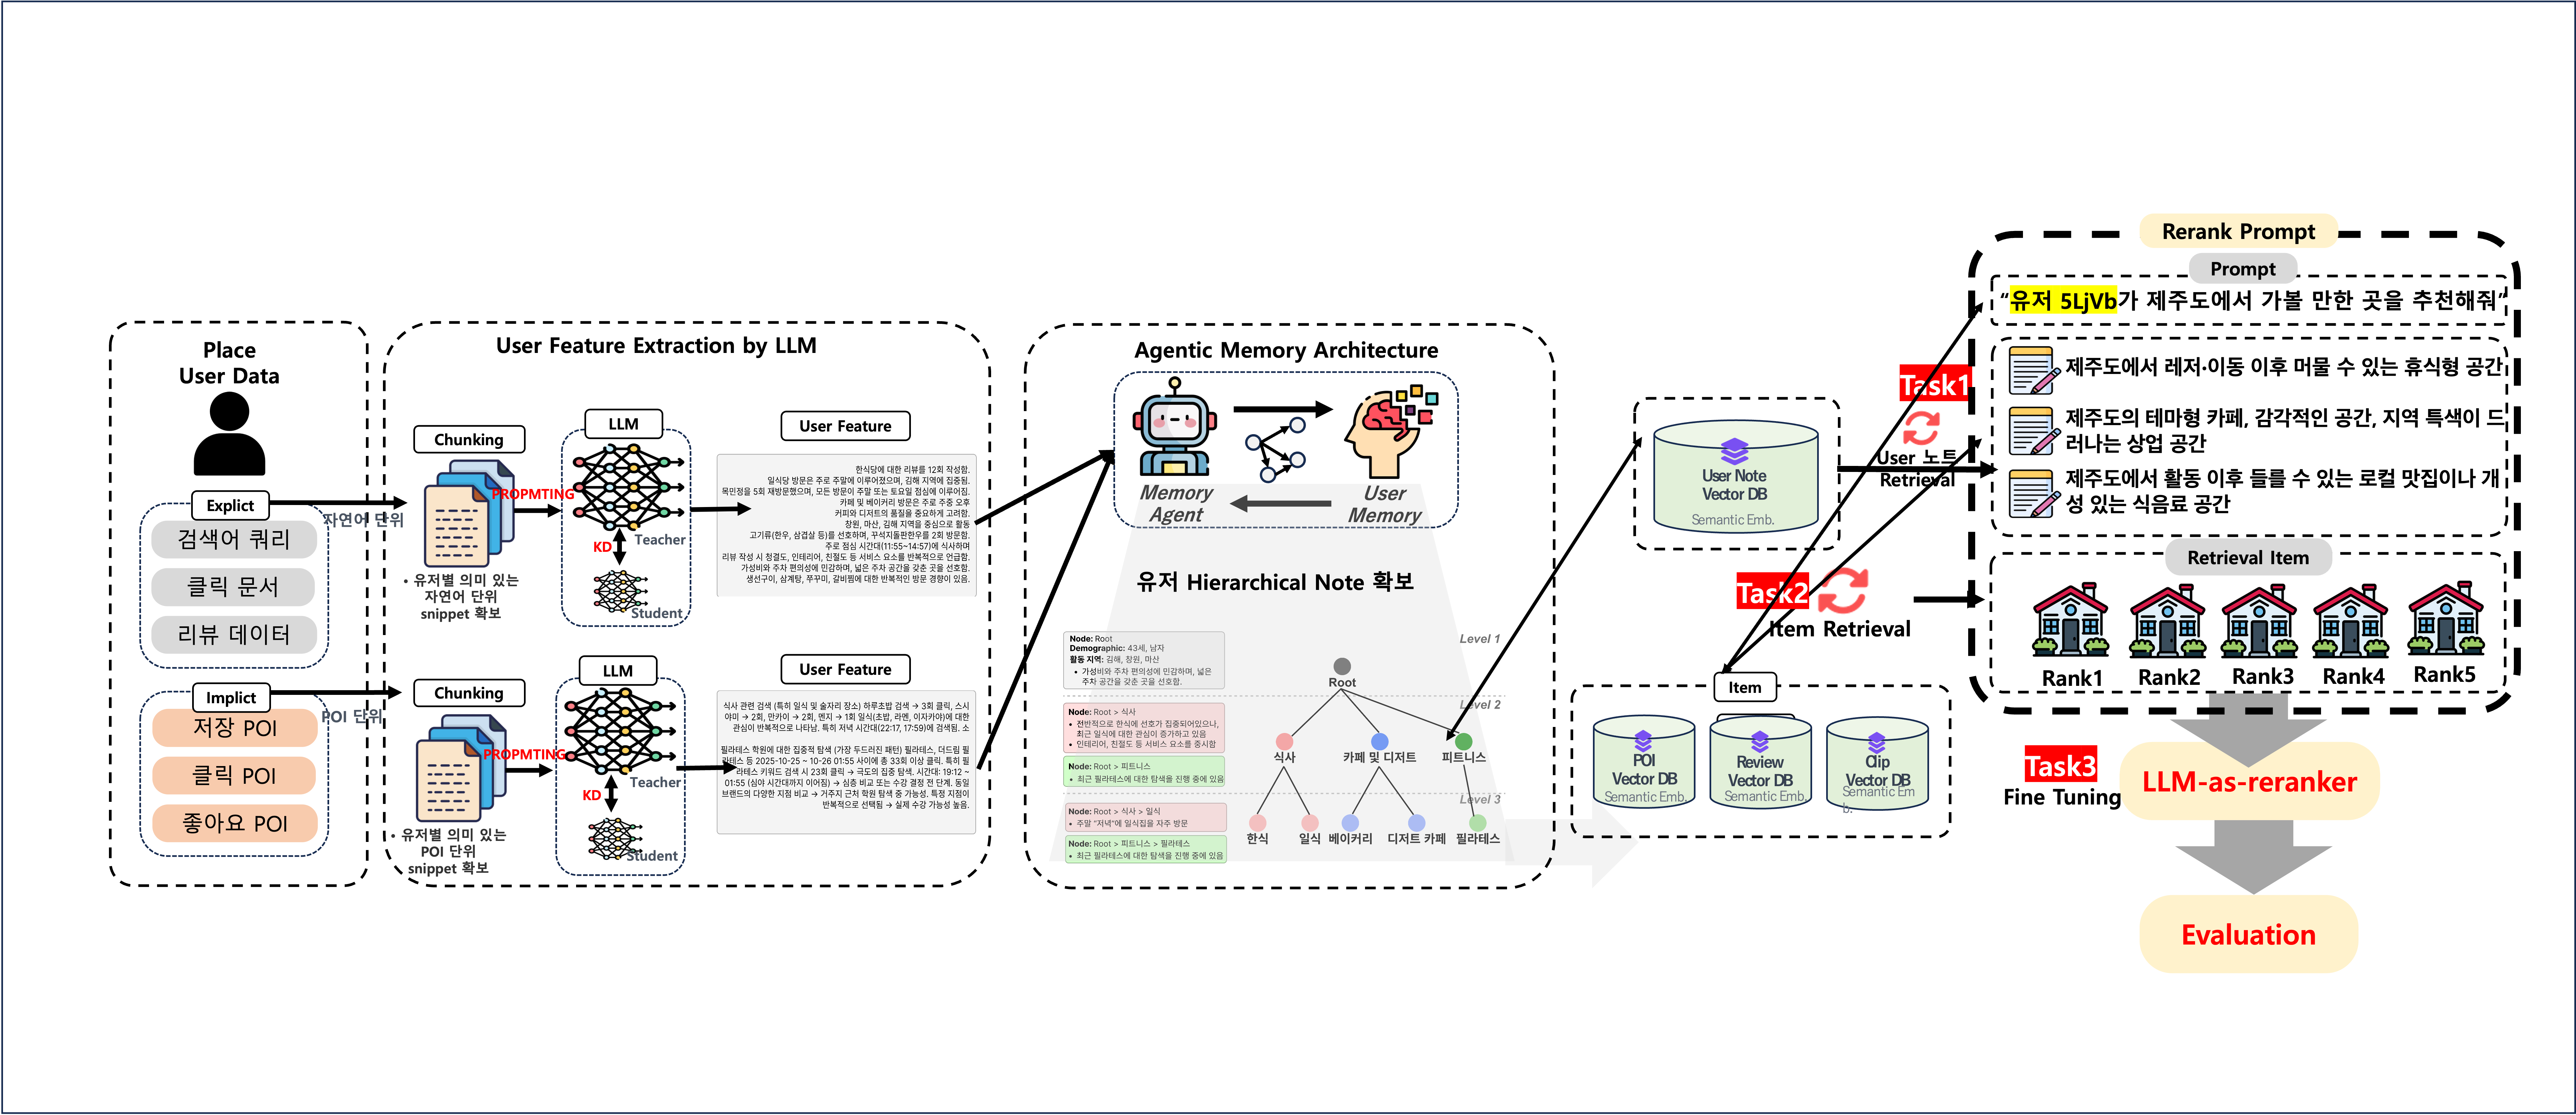
\includegraphics[width=\linewidth]{figures/system-pipeline.png}
  \caption{End-to-end system pipeline. \textit{(1) Signal Extraction}: raw POI interaction logs (search, click, save, review) are processed by an LLM-based feature extractor to produce structured user feature profiles. \textit{(2) Hierarchical Note Memory}: extracted features are routed into a taxonomy-grounded hierarchical note structure maintained by the Memory Agent. \textit{(3) Context-Adaptive Persona Construction}: relevant notes are selectively retrieved and synthesized into a purpose-specific persona. \textit{(4) Persona-Driven Reranking}: the persona is injected into a rerank prompt; an LLM-as-reranker (fine-tuned on POI preference data) produces the final ranked list of candidate places, which is evaluated against ground-truth interactions.}
  \label{fig:pipeline}
\end{figure*}

We propose an end-to-end framework for POI-centric user persona construction and preference-driven place reranking. As illustrated in Figure~\ref{fig:pipeline}, the system consists of four stages: (1)~\textbf{Signal Extraction}, which converts raw POI interaction data---search queries, clicks, saves, and reviews---into structured user feature profiles by separately processing explicit signals (user-written reviews) and implicit signals (behavioral logs); (2)~\textbf{Hierarchical Note Memory}, a persistent, taxonomy-grounded data structure that organizes extracted features into multi-level notes spanning broad lifestyle domains down to fine-grained subcategories; (3)~\textbf{Memory Agent}, an LLM-driven controller that maintains the memory through bidirectional operations---forward aggregation of new signals into appropriate notes, and backward consolidation to preserve structural integrity---and supports \textbf{context-adaptive persona construction} by selectively reading from relevant portions of the hierarchy; and (4)~\textbf{Persona-Driven Reranking}, where the constructed persona is injected into a rerank prompt and an LLM-as-reranker, fine-tuned on POI preference data, produces the final ranked list of candidate places for downstream evaluation.

The remainder of this section describes each component in detail: signal extraction (Section~3.2), the hierarchical note memory structure (Section~3.3), the forward aggregation pass (Section~3.4), the backward consolidation pass (Section~3.5), and persona construction (Section~3.6).

\begin{figure}[t]
  \centering
  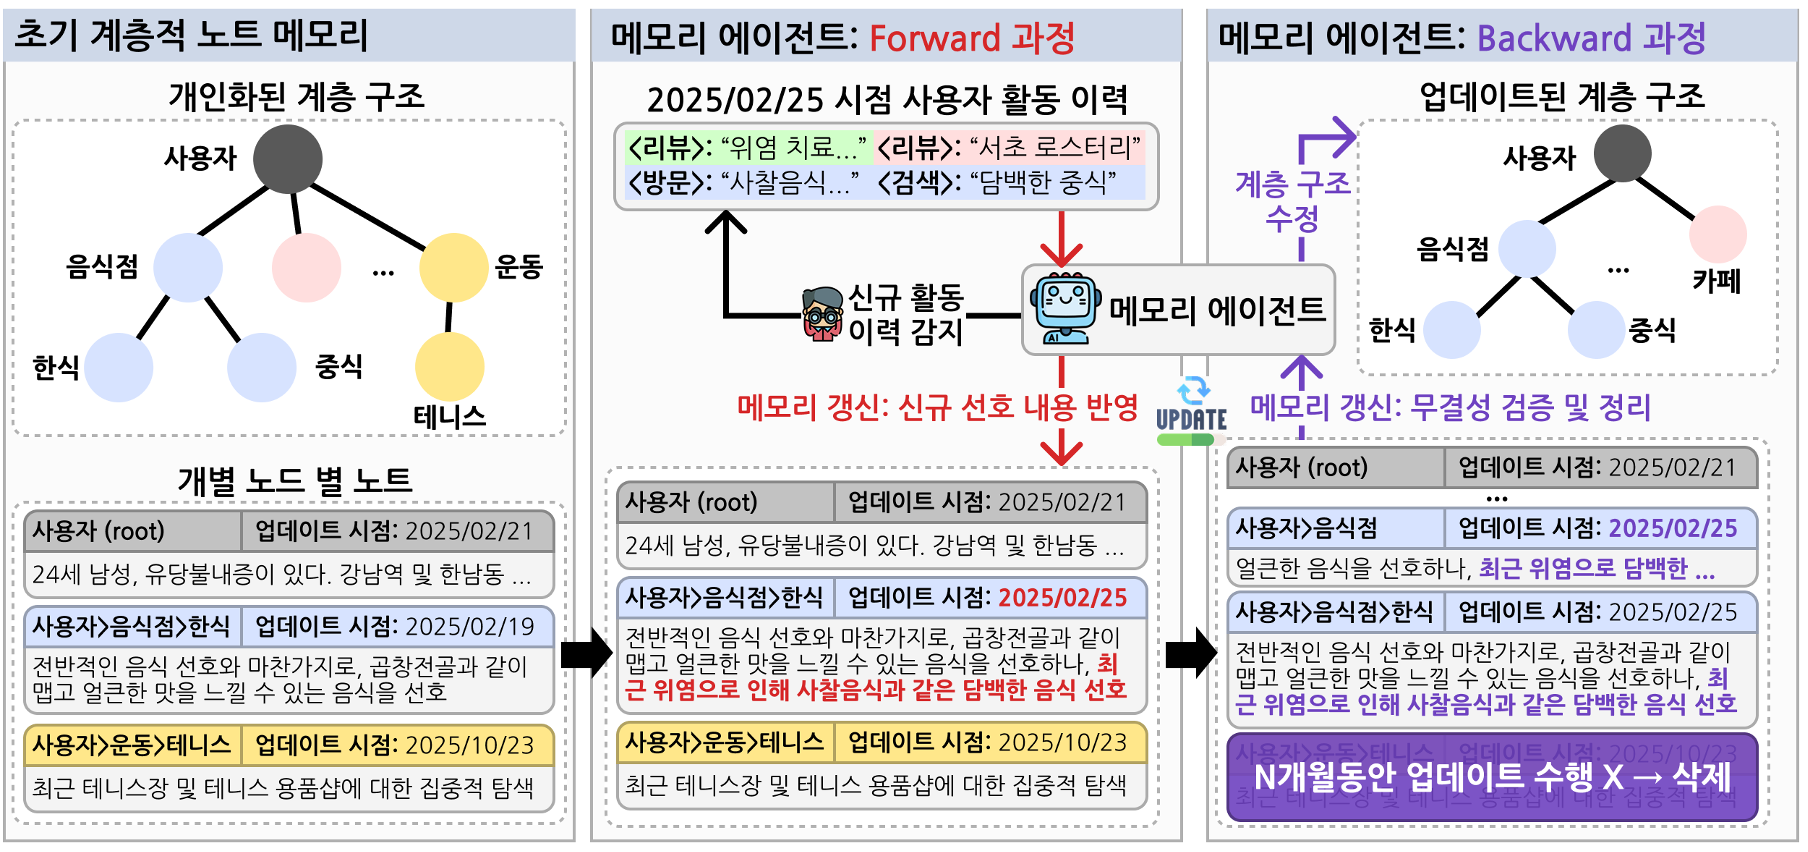
\includegraphics[width=\linewidth]{figures/memory-agent-workflow.png}
  \caption{Illustration of the Memory Agent's forward and backward passes. \textit{Left}: initial hierarchical note memory with per-node notes indexed by POI category. \textit{Center}: the forward aggregation pass detects new user activity, routes extracted preferences to target nodes, and updates note content. \textit{Right}: the backward consolidation pass revises the tree structure, elevates common traits to parent nodes, and prunes stale leaves.}
  \label{fig:workflow}
\end{figure}


\subsection{POI Interaction Signal Extraction}

User preferences toward places manifest through two fundamentally different modalities. We extract structured preference profiles from each modality independently before unifying them within the hierarchical memory. This dual-extraction approach follows the paradigm established by PersonaMem-v2~\cite{personamem-v2}, extended here with a third axis for demographic information and adapted to the POI domain where implicit behavioral signals are particularly abundant.

\subsubsection{Explicit Signal Extraction.}
Explicit signals originate from user-authored content---primarily place reviews---where preferences are stated directly in natural language (e.g., ``I love spicy broth'' or ``the quiet atmosphere was perfect for working''). Similar to the dense extraction approach of DEEPER~\cite{deeper}, we process review histories with an LLM-based extraction pipeline that, for each user, produces a set of structured persona items. Each item consists of four fields: (a)~\textit{User\_Info}, a single atomic fact about the user's lifestyle or preference distilled from the review evidence; (b)~\textit{Rationale}, a chain-of-thought justification grounded in specific review dates, place names, and quoted expressions; (c)~\textit{User\_Vocabulary}, verbatim words and phrases from the user's original text to preserve linguistic identity; and (d)~\textit{Reference}, indices into the source review records.

To handle the wide variance in review volume across users, we employ two few-shot prompt strategies: a \textit{rich} variant with detailed examples for users who have written many reviews, and a \textit{sparse} variant with conservative, observation-oriented examples for users with limited review data. The sparse strategy deliberately avoids over-generalizing from insufficient evidence, instead emphasizing factual descriptions of observed behavior.

\subsubsection{Implicit Signal Extraction.}
Implicit signals are derived from non-verbal behavioral traces: search queries, POI clicks, dwell patterns, and place saves. Unlike reviews, these actions do not directly articulate preferences, but consistent patterns across many interactions can reveal latent interests~\cite{proex}. We construct a profiling pipeline that transforms raw click logs into structured personas through the following steps:

\begin{enumerate}
    \item \textbf{Sessionization.} Consecutive interactions involving the same query or the same POI within a 60-minute window are grouped into micro-sessions. Each session records the query text, timestamps, day of week, clicked POI name and category, location, review popularity rank, and click count.

    \item \textbf{Demographic context attachment.} Available demographic attributes (age, gender, marital status, household composition, occupation, and children information) are prepended to the session log as structured metadata. These attributes are later routed exclusively to the root node's \texttt{user\_info} field during hierarchical path mapping (Section~3.4), enforcing a clean separation between demographic facts and behavioral preferences.

    \item \textbf{LLM-based persona profiling.} The sessionized log is passed to an LLM with strict constraints: (a)~all persona claims must cite specific click evidence; (b)~hallucination of unobserved behaviors (e.g., inferring residence from visit locations) is prohibited; (c)~stereotypical reasoning based on demographics is forbidden; and (d)~the output must decompose preferences into predefined POI domains (dining, caf\'{e}s, travel, medical, beauty, shopping, etc.).
\end{enumerate}

The output is a domain-partitioned persona string, where each domain section describes the user's inferred preferences with concrete behavioral evidence. To capture temporal dynamics, we apply this extraction over sliding windows (e.g., 21-day periods) across the observation period and aggregate the per-window results into a unified implicit persona per user.


\subsection{Hierarchical Note Memory Structure}

The core data structure is a three-level tree grounded in a predefined POI taxonomy, designed to support preference representation at multiple levels of abstraction. This structure extends the three-level paradigm of PersonaMem-v2~\cite{personamem-v2} with domain-specific customization for POI services and dynamic path management.

\subsubsection{POI Taxonomy.}
The base hierarchy defines Level~1 as the root node (representing the user as a whole), Level~2 as broad POI domains, and Level~3 as fine-grained subcategories within each domain. The predefined taxonomy includes 11 Level~2 domains---\textit{Dining}, \textit{Caf\'{e}/Dessert}, \textit{Transportation/Mobility}, \textit{Travel/Accommodation}, \textit{Leisure/Sports}, \textit{Culture/Arts}, \textit{Self-development}, \textit{Pets}, \textit{Shopping}, \textit{Medical}, and \textit{Beauty}---each containing 2--10 Level~3 subcategories (e.g., Dining $\rightarrow$ \{Korean, Japanese, Chinese, Western, Fast Food, \ldots\}). Unlike the fixed-slot approach of PersonaMem-v2, the Memory Agent may dynamically extend this taxonomy by creating new Level~3 nodes when user data warrants categories not present in the base hierarchy, subject to hierarchical consistency constraints described in Section~3.4. A maximum depth of three levels is enforced both at the prompt level and through structural validation.

\subsubsection{Note Schema.}
Each node in the hierarchy is associated with a \textit{Note}, a structured record that stores the accumulated preference knowledge for that category. A note contains the following fields:

\begin{itemize}
    \item \textbf{path}: the full hierarchical path (e.g., ``User $>$ Dining $>$ Korean''),
    \item \textbf{user\_info}: demographic and factual attributes (populated \textit{only} at the root node; all sub-nodes are constrained to empty lists),
    \item \textbf{summary}: a natural-language paragraph summarizing the user's preferences and behavioral patterns for this category, integrating both explicit and implicit signals,
    \item \textbf{keywords}: BM25-oriented keyword tags for retrieval,
    \item \textbf{updated\_count}: the number of times the note content has been substantively modified,
    \item \textbf{recently\_updated}: the date of the most recent content update.
\end{itemize}

All notes for a user are stored atomically in a single Parquet file, enabling efficient bulk I/O. The tree structure metadata (parent-child relationships, node levels) is maintained in a separate hierarchy file. This separation allows the Memory Agent to load, modify, and persist the entire memory state in a single read-modify-write cycle per operation.


\subsection{Memory Agent: Forward Aggregation}

When new interaction data arrives (either explicit persona extractions or implicit persona profiles), the Memory Agent executes a three-step forward pass to integrate the information into the existing memory. Each step is mediated by an LLM call, resulting in $2 + N$ total calls per user, where $N$ is the number of distinct target paths identified in Step~2.

\subsubsection{Step~1: Preference Profile Extraction.}
The raw interaction text---combining both implicit behavioral profiles and explicit review extractions---is analyzed by an LLM to separate three categories of information:

\begin{itemize}
    \item \textbf{User information} ($\mathcal{U}$): objective, slowly-changing facts such as age, occupation, and primary activity region.
    \item \textbf{Explicit preferences} ($\mathcal{P}_e$): stated preferences where the user directly expresses likes, dislikes, or requirements in language (e.g., ``I prefer acidic coffee'' or ``I look for outlets at caf\'{e}s'').
    \item \textbf{Implicit preferences} ($\mathcal{P}_i$): latent preferences inferred from non-verbal behavioral patterns (e.g., ``tends toward isolated, productivity-oriented spaces'' derived from repeated clicks on quiet study caf\'{e}s).
\end{itemize}

This three-axis separation extends the two-axis approach of PersonaMem-v2~\cite{personamem-v2} (which combines demographics with explicit preferences) by isolating demographic facts into a dedicated channel. The LLM is instructed to preserve concrete keywords from the source data rather than abstracting them (e.g., extracting specific dish names rather than ``diverse menu''), to merge semantically similar items into compact statements, and to strictly distinguish between exploratory actions (clicks, searches) and confirmed actions (visits, reservations) to avoid inflating behavioral claims.

\subsubsection{Step~2: Hierarchical Path Mapping.}
The extracted preference items are mapped to target paths in the hierarchy through context-aware routing. The LLM receives the extracted profile along with both the base taxonomy paths and any existing user-specific paths, and assigns each item to the most appropriate node. This mapping follows several principles:

\begin{enumerate}
    \item \textbf{Root exclusivity for demographics}: User information items ($\mathcal{U}$) are mapped exclusively to the root node's \texttt{user\_info} field. Creating subcategory nodes for demographic attributes (e.g., ``User $>$ Region'') is strictly prohibited.

    \item \textbf{Context-aware routing}: Preference items are routed based on their semantic context. For example, ``prefers quiet atmosphere'' is mapped to ``User $>$ Caf\'{e}'' if the surrounding evidence is caf\'{e}-related, but to the root node if it reflects a general cross-domain tendency.

    \item \textbf{Semantic reuse}: Existing paths are preferred over creating new ones when they can semantically subsume the new item (e.g., a ``latte'' preference maps to an existing ``Coffee/Tea'' node rather than creating a new ``Latte'' sibling).

    \item \textbf{Hierarchical consistency}: New Level~3 nodes must match the abstraction level of their siblings---e.g., ``Korean'' and ``Japanese'' are valid siblings under ``Dining'', but ``Naengmyeon'' (a specific dish) is not, as it belongs under ``Korean'' or a similar subcategory. Nodes at Level~4 or deeper are prohibited. Node names must represent place categories, not user behavioral patterns.

    \item \textbf{Aggregation}: Items targeting the same path are grouped into a single assignment object containing both explicit and implicit preference lists, ensuring one LLM update call per path.
\end{enumerate}

\subsubsection{Step~3: Note Update.}
For each target path with new data, the Memory Agent invokes an LLM to merge the incoming preferences with the existing note content. The LLM acts as an \textit{editor} rather than a simple appender: it compares new data against existing content, resolves conflicts by favoring more recent information, removes outdated or erroneous entries, and consolidates redundant statements. This active editing approach distinguishes our system from append-only memory designs~\cite{mem0}. The update is differentiated by node role---the root node actively manages user demographics in its \texttt{user\_info} field, while all sub-nodes are prohibited from storing demographic information and focus exclusively on category-specific preferences. When the LLM produces substantive changes to a note, the \texttt{updated\_count} is incremented and the \texttt{recently\_updated} timestamp is refreshed.


\subsection{Memory Agent: Backward Consolidation}

Over time, repeated forward passes may introduce redundancy across sibling nodes, scatter shared preferences across leaf notes, or leave stale nodes from transient interests. The backward consolidation pass addresses these issues through three sequential operations, executed in a specific order: merging first reduces the number of siblings, which yields clearer common traits for the subsequent elevation step, and pruning last removes nodes that may have become stale after reorganization.

\subsubsection{Sibling Node Merging.}
For each parent node with two or more children, the Memory Agent presents all child notes to an LLM and asks it to identify semantically overlapping siblings that should be merged. Only leaf nodes (those without children of their own) are eligible for merging. When a merge is approved, the LLM produces a unified \texttt{merged\_note} that integrates the content of the source nodes, removing duplication while preserving unique details. The merged note inherits the cumulative \texttt{updated\_count} and the most recent timestamp from its sources. Source nodes are then deleted from both the note store and the hierarchy. If a source node is only partially consumed by the merge (i.e., some of its content belongs to a different thematic cluster), the LLM also produces an \texttt{updated\_source} with the remaining content, which is written back to the original node.

\subsubsection{Common Trait Elevation.}
After merging, the Memory Agent examines each parent--children group to identify preferences that appear across two or more sibling notes. An LLM extracts these common traits and rewrites the parent note to incorporate them, while simultaneously rewriting each child note to remove the elevated content.

This operation enforces a hierarchical invariant: shared preferences reside at the appropriate abstraction level, not duplicated across subcategories. Cross-subcategory tendencies (e.g., a general preference for spicy food) belong at the domain level (``Dining''), not replicated in ``Korean,'' ``Chinese,'' and ``Asian'' subcategory notes. The process respects level semantics: the root node absorbs user-wide commonalities, Level~2 nodes absorb domain-wide patterns, and Level~3 nodes retain only subcategory-specific details.

Formally, this operation can be understood as minimizing the total description length across the tree. Let $C(n)$ denote the content of note $n$, $\text{pa}(n)$ its parent, and $\text{sib}(n)$ its siblings. Common trait elevation identifies the mutual information $I = C(n_i) \cap C(n_j)$ shared among siblings $n_i, n_j \in \text{children}(\text{pa}(n))$ and restructures the tree so that:
\begin{equation}
    C'(\text{pa}(n)) = C(\text{pa}(n)) \cup I, \quad C'(n_k) = C(n_k) \setminus I \quad \forall\, n_k \in \text{children}(\text{pa}(n))
\end{equation}
This reduces the total storage $\sum_n |C(n)|$ by $|(|\text{children}| - 1) \cdot I|$, achieving hierarchical compression analogous to the Minimum Description Length principle~\cite{mdl}. To our knowledge, this explicit trait elevation operation has not been proposed in prior memory systems~\cite{mem0,amem,personamem-v2,emem}.

\subsubsection{Stale Leaf Pruning.}
Finally, the Memory Agent removes leaf nodes that represent transient or exploratory interests that did not develop into sustained preferences. A leaf node $n$ is pruned if it satisfies two conditions simultaneously:
\begin{equation}
    \texttt{updated\_count}(n) \leq \tau_u \quad \text{and} \quad \texttt{age}(n) > \tau_d
\end{equation}
where $\tau_u$ is the minimum update threshold (default: 2) and $\tau_d$ is the staleness threshold in days (default: 120). Nodes are processed in decreasing depth order so that pruning a leaf may expose its parent as a new leaf, which is then evaluated in the same pass. This mechanism prevents the memory from accumulating noise from one-off exploratory behaviors while retaining nodes that have been reinforced through repeated interactions.


\subsection{Context-Adaptive Persona Construction}

The hierarchical memory enables flexible, purpose-driven persona generation, distinguishing our approach from flat persona representations that must either include all information (risking dilution) or rely on ad-hoc filtering~\cite{persona-db}. Given a recommendation context (e.g., ``dining recommendation for a weekend trip'' or ``caf\'{e} suggestion near the office''), the persona construction proceeds in two steps:

\begin{enumerate}
    \item \textbf{Path Selection.} An LLM receives the full set of available hierarchy paths and the stated purpose, then selects 3--8 paths whose content is most relevant to the recommendation scenario. This selective reading avoids overwhelming the persona with irrelevant details and naturally adapts the granularity: a dining-specific query draws on ``Dining'' subtree paths, while a general lifestyle query may draw on the root and multiple Level~2 nodes.

    \item \textbf{Persona Synthesis.} The notes at the selected paths are passed to an LLM, which synthesizes a concise persona consisting of a one-sentence overview, approximately five key preference traits, and approximately three behavioral patterns. The persona is expressed in natural language suitable for direct injection into a downstream recommendation or search prompt.
\end{enumerate}

Because the memory stores preferences at multiple abstraction levels and separates them by POI category, different purposes can yield qualitatively different personas for the same user---a dining persona may emphasize cuisine preferences and meal timing, while a travel persona highlights accommodation style and activity interests.


%% ============================================================
%% EXPERIMENTS (SKELETON)
%% ============================================================
\section{Experiments}

\subsection{Experimental Setup}

\subsubsection{Dataset.}
We evaluate on anonymized POI interaction logs from a large-scale map service, comprising click, save, search, and review data. We sample users with sufficient interaction volume and split temporally: interactions before a cutoff date are used for memory construction, and subsequent interactions serve as ground truth for evaluation.

\subsubsection{Baselines.}
We compare against five baselines spanning the design space:
\begin{itemize}
    \item \textbf{No-Memory}: LLM with only current session context (lower bound).
    \item \textbf{Full-Context}: All raw interaction logs placed in the LLM context window (quality upper bound, impractical at scale).
    \item \textbf{Flat-Memory}: Mem0-style~\cite{mem0} flat list with ADD/UPDATE/DELETE operations (tests hierarchy value).
    \item \textbf{Fixed-Hierarchy}: PersonaMem-v2-style~\cite{personamem-v2} three-level tree with predefined fixed slots (tests dynamic routing value).
    \item \textbf{Ours (full)}: Dynamic routing + common trait elevation + three-axis separation.
\end{itemize}

\subsubsection{Ablation Variants.}
To isolate the contribution of each proposed component:
\begin{itemize}
    \item \textbf{$-$dynamic}: Replace dynamic routing with fixed predefined slots.
    \item \textbf{$-$elevation}: Remove common trait elevation from the backward pass.
    \item \textbf{$-$3axis}: Merge demographics into the preference channel (two-axis, as in PersonaMem-v2).
    \item \textbf{$-$backward}: Remove the entire backward consolidation pass.
    \item \textbf{$-$implicit}: Use only explicit (review) signals.
    \item \textbf{$-$explicit}: Use only implicit (behavioral) signals.
\end{itemize}

\subsubsection{Evaluation Metrics.}
We measure along three dimensions:
\begin{itemize}
    \item \textbf{Quality}: Preference prediction accuracy (given memory, predict next POI category; Accuracy@$k$, MRR), persona consistency score adapted from PersonaGym~\cite{personagym}, and downstream recommendation metrics (HR@$k$, NDCG@$k$).
    \item \textbf{Efficiency}: Tokens consumed per user, LLM API calls per user, wall-clock latency per user, and cost per user per day.
    \item \textbf{Structural health}: Average tree depth, node count per user, stale node ratio, and merge rate over time.
\end{itemize}


\subsection{Main Results}

% TODO: Insert main comparison table (baselines vs ours)

\subsection{Ablation Study}

% TODO: Insert ablation table showing contribution of each component

\subsection{Scalability Analysis}

% TODO: Token cost, latency, and scaling curves

\subsection{Qualitative Analysis}

% TODO: Example memory trees, persona outputs, failure cases


%% ============================================================
%% LIMITATIONS AND FUTURE WORK
%% ============================================================
\section{Limitations and Future Work}

\textbf{Cross-node linking.}
Our tree hierarchy does not capture relationships between nodes in different branches (e.g., ``morning person'' in the lifestyle branch and ``caf\'{e} lover'' in the dining branch). A-Mem~\cite{amem} demonstrates that such cross-node activation links significantly improve multi-hop reasoning. Incorporating inter-branch connections while preserving the compression benefits of trait elevation is a promising direction.

\textbf{LLM dependence.}
All memory operations (extraction, routing, update, merging, elevation) rely on LLM judgment. Dynamic path creation and common trait identification are enforced through prompt instructions rather than algorithmic guarantees. Future work could introduce hybrid approaches combining LLM reasoning with information-theoretic thresholds (e.g., keyword overlap ratios for trait commonality detection).

\textbf{Scalability.}
The forward pass requires $2 + N$ LLM calls per user (where $N$ is the number of target paths), and implicit extraction averages 73K input tokens per user. At 10K users per day, this represents a substantial computational cost. Knowledge distillation to smaller models~\cite{personamem-v2} and input clustering~\cite{personax} are viable paths to reduce this overhead by an estimated 7--50$\times$.

\textbf{Language specificity.}
All prompts in the current system are written in Korean, and the POI taxonomy reflects Korean place categories. Generalization to other languages and cultural contexts requires taxonomy adaptation and prompt translation, which we leave to future work.


%% ============================================================
%% CONCLUSION
%% ============================================================
\section{Conclusion}

We presented a POI-centric hierarchical note-based memory system for constructing and maintaining user place personas. By extending the hierarchical memory paradigm with dynamic routing, common trait elevation, and three-axis preference separation, the proposed system enables structured, multi-level preference modeling that evolves with user behavior. The bidirectional Memory Agent---performing forward aggregation and backward consolidation---maintains temporal consistency and structural integrity without manual intervention. Our evaluation framework and experimental results demonstrate improvements over full-context, flat-memory, and fixed-hierarchy baselines on both persona quality and downstream recommendation metrics, while operating at substantially lower computational cost.


%% ============================================================
%% REFERENCES
%% ============================================================
\bibliographystyle{ACM-Reference-Format}

\begin{thebibliography}{99}

\bibitem{personamem-v2}
X.~Hu, H.~Wu, Y.~Hu, et~al.
\newblock PersonaMem-v2: Hierarchical agentic memory for personalized {LLM} agents.
\newblock In \textit{Proceedings of AAAI}, 2025.

\bibitem{personamem}
X.~Hu et~al.
\newblock PersonaMem: A structured memory approach for personalized language model agents.
\newblock \textit{arXiv preprint}, 2024.

\bibitem{mem0}
D.~Yadav et~al.
\newblock Mem0: Building production-ready {AI} agents with scalable long-term memory.
\newblock \textit{arXiv preprint arXiv:2504.19413}, 2025.

\bibitem{amem}
W.~Xu, Z.~Liang, et~al.
\newblock A-Mem: Agentic memory for {LLM} agents.
\newblock \textit{arXiv preprint arXiv:2502.12110}, 2025.

\bibitem{emem}
Various.
\newblock EMem: Expectation-guided memory for long-horizon agents.
\newblock \textit{arXiv preprint arXiv:2511.17208}, 2025.

\bibitem{memgpt}
C.~Packer et~al.
\newblock MemGPT: Towards {LLMs} as operating systems.
\newblock \textit{arXiv preprint}, 2023.

\bibitem{beyond-context-window}
Various.
\newblock Beyond the context window: Long-context {LLMs} vs memory-augmented agents.
\newblock \textit{arXiv preprint arXiv:2603.04814}, 2025.

\bibitem{lost-in-the-middle}
N.~F.~Liu, K.~Lin, J.~Hewitt, A.~Paranjape, M.~Bevilacqua, F.~Petroni, and P.~Liang.
\newblock Lost in the middle: How language models use long contexts.
\newblock \textit{Transactions of the ACL}, 2024.

\bibitem{personahub}
G.~Liu et~al.
\newblock PersonaHub: A large-scale world simulator for persona-driven {LLM} agents.
\newblock \textit{arXiv preprint arXiv:2407.18899}, 2024.

\bibitem{personagym}
V.~Samuel et~al.
\newblock PersonaGym: A dynamic evaluation framework for persona agents.
\newblock \textit{arXiv preprint arXiv:2407.18416}, 2024.

\bibitem{personabench}
Various.
\newblock PersonaBench: Benchmarking persona-based language agents.
\newblock \textit{arXiv preprint arXiv:2407.17960}, 2024.

\bibitem{deeper}
Various.
\newblock DEEPER: Dense extraction of personalized expressions for recommendations.
\newblock \textit{arXiv preprint}, 2024.

\bibitem{synthesizeme}
Various.
\newblock SynthesizeMe: Personalized language model adaptation via profile-conditioned synthesis.
\newblock \textit{arXiv preprint}, 2024.

\bibitem{proex}
Various.
\newblock ProEx: Expert-level preference extraction from user behavior.
\newblock \textit{arXiv preprint}, 2024.

\bibitem{zeropoirec}
Various.
\newblock ZeroPOIRec: Zero-shot {POI} recommendation with {LLM}-generated personas.
\newblock \textit{arXiv preprint}, 2024.

\bibitem{persona-db}
Various.
\newblock Persona-DB: Efficient large language model personalization for response prediction.
\newblock In \textit{Findings of ACL}, 2024.

\bibitem{rmm}
Various.
\newblock RMM: Retrieval-augmented memory for personalized dialogue.
\newblock \textit{arXiv preprint}, 2024.

\bibitem{personax}
Various.
\newblock PersonaX: Persona-driven user behavior clustering for large-scale recommendation.
\newblock \textit{arXiv preprint}, 2024.

\bibitem{dpr}
V.~Karpukhin et~al.
\newblock Dense passage retrieval for open-domain question answering.
\newblock In \textit{Proceedings of EMNLP}, 2020.

\bibitem{contriever}
G.~Izacard et~al.
\newblock Unsupervised dense information retrieval with contrastive learning.
\newblock \textit{TMLR}, 2022.

\bibitem{mdl}
P.~Gr{\"u}nwald.
\newblock \textit{The Minimum Description Length Principle}.
\newblock MIT Press, 2007.

\end{thebibliography}

\end{document}
